\chapter{Particle Identification}

\section{Introduction}
Following on from the process of clustering hits together into associated groups, and fitting tracks to obtain parameters such as the slope or particle momentum, it is essential to be able to determine the nature of the particle that produced those hits.

For \ac{CCQE} neutrino interactions it is of critical importance to be able to identify the flavour of the lepton that was produced, and to be able to associate a track with the passage of a muon (if the interaction involved a $\nu_\mu$). Muon identification is often performed with the help of small detector units around the sides of the main detector. A muon typically behaves as a minimum ionising particle, and will often travel all the way through a detector and leave through one of the sides. A signal in such a muon detector is a strong indicator that the track leading into it was produced by a muon.

In the case of a \ac{LAr TPC}, the aim is to fully contain muons (at least, if they are produced somewhere near the centre of the detector volume), and identification must be performed using information from the track reconstruction stage. For the simplest category of charged current interactions, the muon should be represented by the longest track visible in the event, and it is on this basis that the primary identification of muon tracks will be carried out.

For other types of interaction, or for electron neutrinos, there is a much greater chance of an electromagnetic or hadronic shower developing in the event. One advantage often claimed of LAr TPCs is the ability to achieve electron--pion separation by looking at the rate of energy loss, $dE/dx$.

\section{Muon Track Identification}
In order to be able to select muons based on the track length (approximated as the number of hits contained), it is useful to know the distributions of track lengths for various particle types which may be present in the charged current interactions considered. 

\subsection{$770\MeV$ $\nu_\mu \rightarrow \mu + p$ (CCQE) Interactions}
This study begins by looking at those distributions for the products of charged current interactions of $770\MeV$ $\nu_\mu$ which produced $\mu + p$ or $\mu + p + \pi^+$ final states, making use of the truth information saved by the simulation. Figure \ref{fig:ccqe-track-lengths-770MeV} shows the distribution of lengths (in terms of number of hits) for muon and proton tracks, and figure \ref{fig:ccqe-electron-lengths-770MeV} shows the distribution of lengths for electron tracks, which are plotted on a different graph because the total number of electron tracks is extremely large, though nearly all such tracks have fewer than 50 hits. These correspond to the delta electrons produced along the length of the other tracks. At neutrino energies around $770\MeV$, there is a strong case to be made for treating all tracks longer than $1000$ hits as muons, resulting in a trade-off between selection efficiency for muons and contamination by protons.

Since the electron tracks are produced arbitrarily along the muon track, it is impossible to eliminate electron hits from the muon track, even with clustering techniques such as those provided by the cellular automaton (see chapter \ref{chapter:CellularAutomaton}). The purity of any such tracks will therefore be reduced by the presence of hits from these short delta electron tracks.

\begin{figure}
\centering
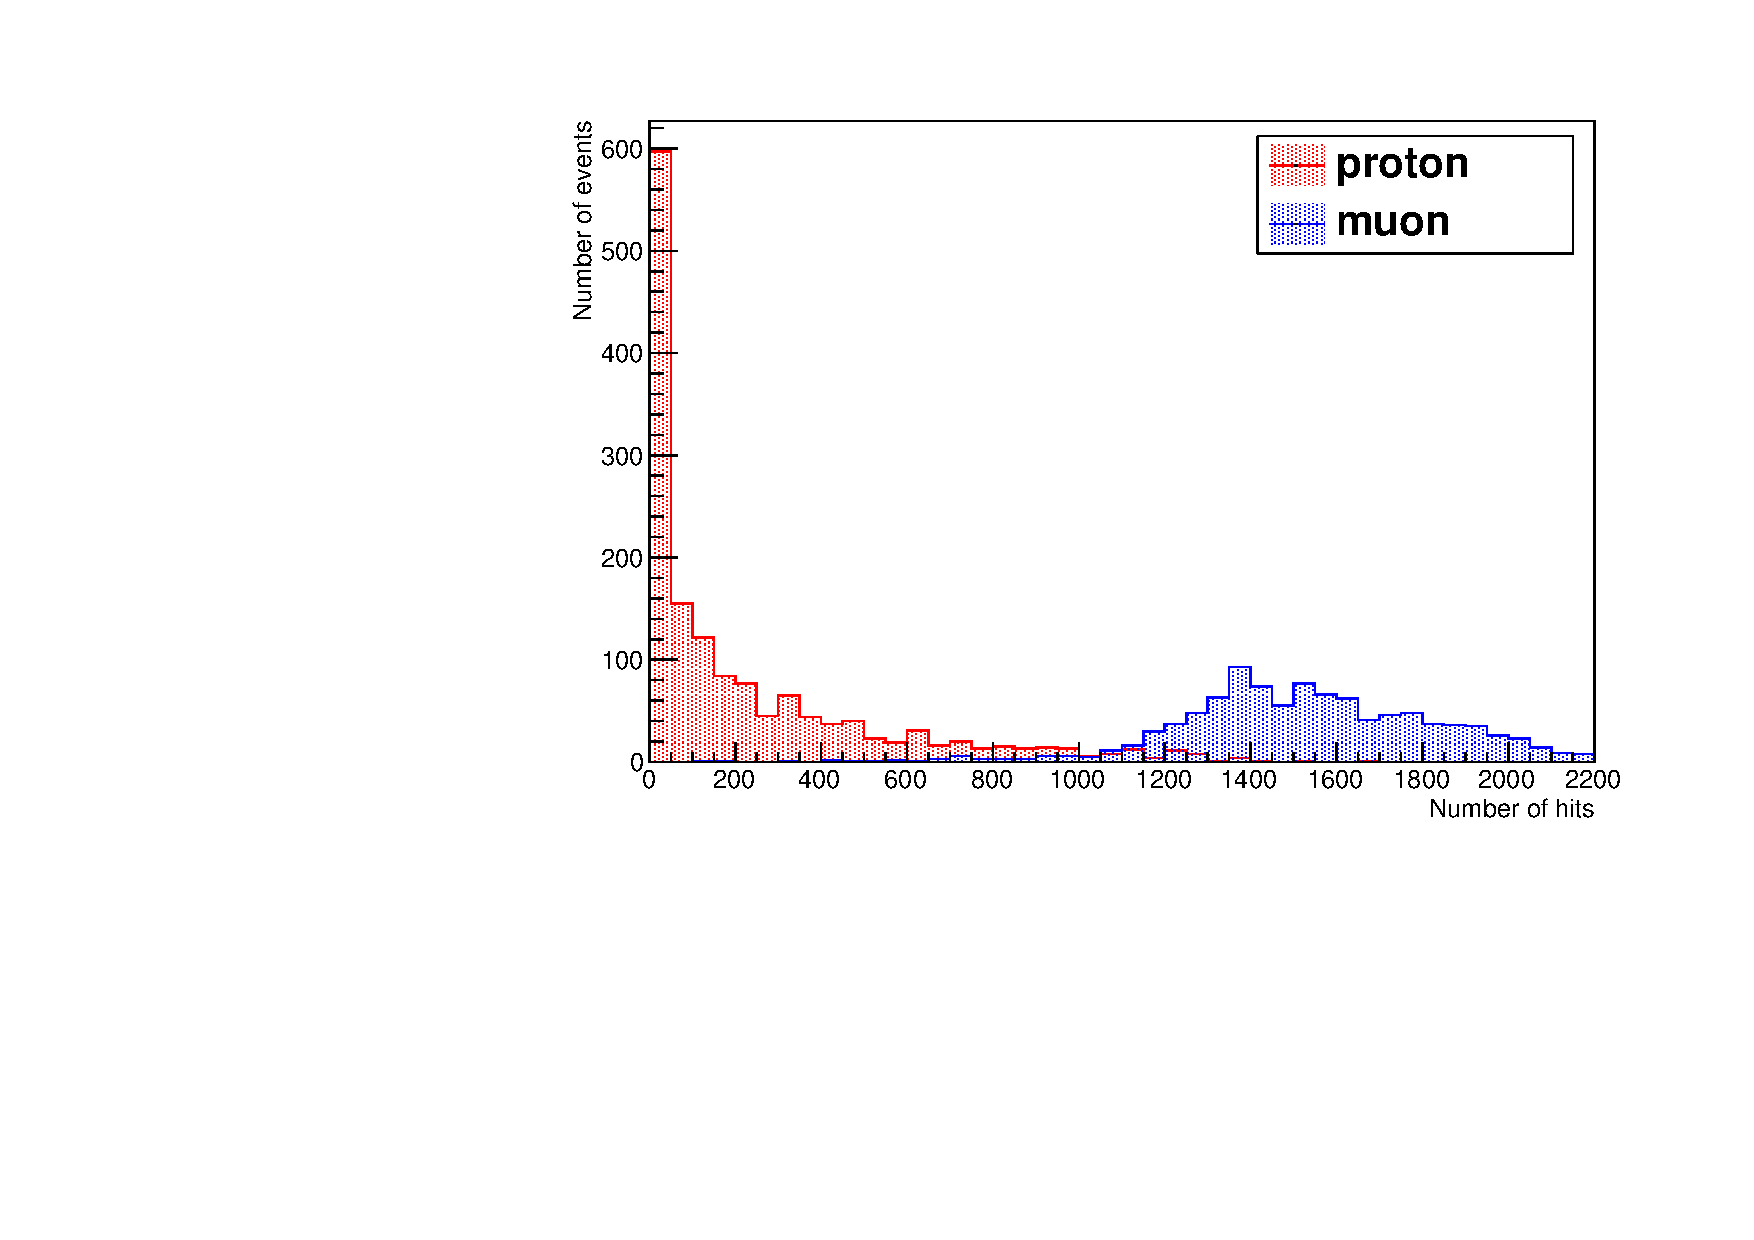
\includegraphics[angle=-90,width=\textwidth]{chapters/particleid_images/particle-lengths-ccqe-770}
\caption[Track length distribution for $\mu$ and $p$ from $770\MeV$ neutrinos (CCQE)]{\label{fig:ccqe-track-lengths-770MeV}Distribution of track lengths, represented as number of hits contained in a track, for muon (blue) and proton (red) tracks produced in charged current interactions of $\nu_\mu$ at $770\MeV$. The distributions are naturally separated at around $1000$ hits.}
\end{figure}

\begin{figure}
\centering
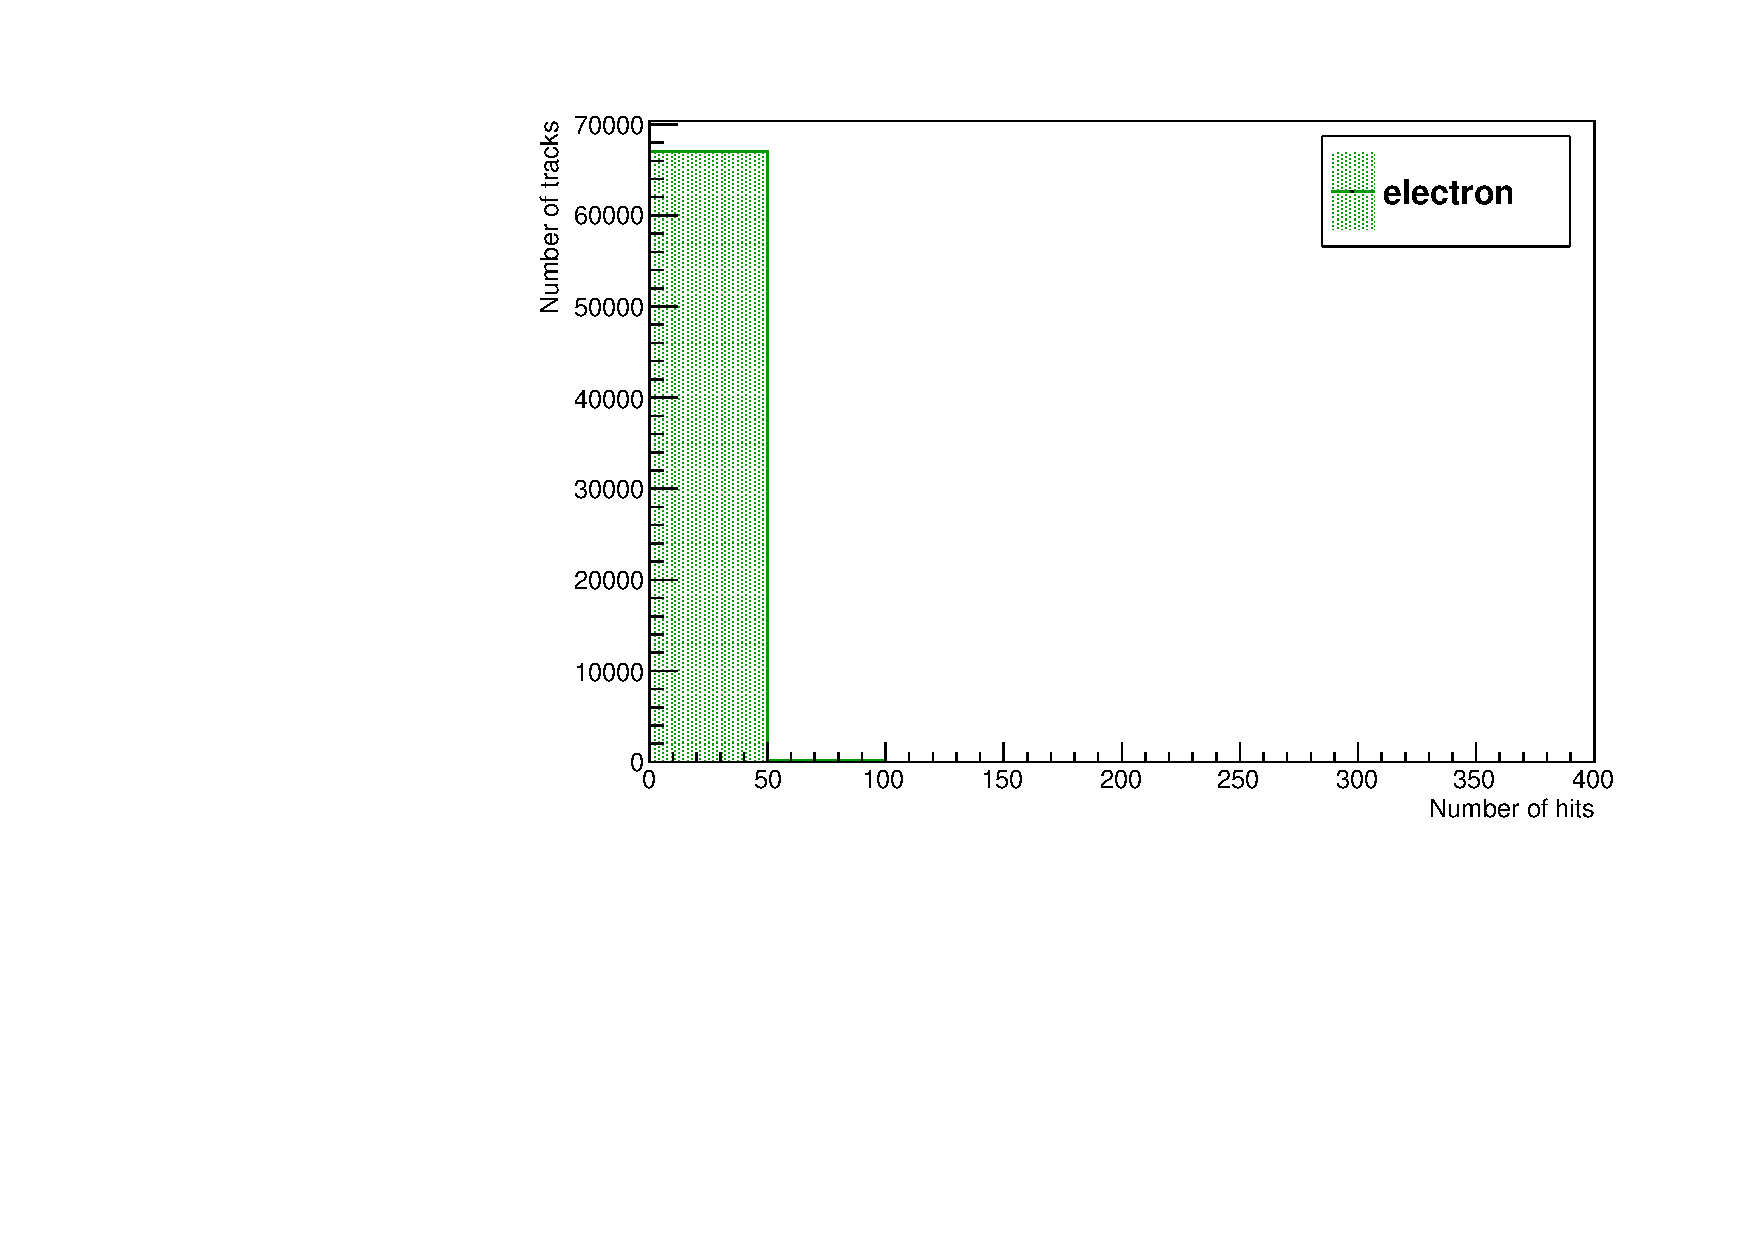
\includegraphics[angle=-90,width=\textwidth]{chapters/particleid_images/electron-lengths-ccqe-770}
\caption[Track length distribution for $e^{-}$ from $770\MeV$ neutrinos (CCQE)]{\label{fig:ccqe-electron-lengths-770MeV}Distribution of track lengths, represented as number of hits contained in a track, for electron tracks produced as secondary particles following charged current interactions of $\nu_\mu$ at $770\MeV$. An extremely large number of very short electron tracks can be seen, corresponding to the production of delta electrons along the length of the trajectories of the primary muon and proton. Most electron tracks have fewer than 50 hits.}
\end{figure}

\subsection{$770\MeV$ $\nu_\mu \rightarrow \mu + p + \pi^+$ (CCPi) Interactions}
This data set contains 1000 events where a $770\MeV$ $\nu_\mu$ underwent a charged current interaction with an Argon nucleus, producing a $\mu + p + \pi^+$ final state. The distribution of track lengths (represented in terms of the number of hits) for muons, protons and charged pions is shown in figure \ref{fig:ccpi-track-lengths-770MeV} and for electrons in figure \ref{fig:ccpi-electron-lengths-770MeV}. Here, the separation of muons from other particles by track length alone is not a realistic proposal; although the muons dominate the longer tracks, a number of pion tracks are also long enough to provide significant pollution of the muon selection if track length alone is used to discriminate particle type.

\begin{figure}
\centering
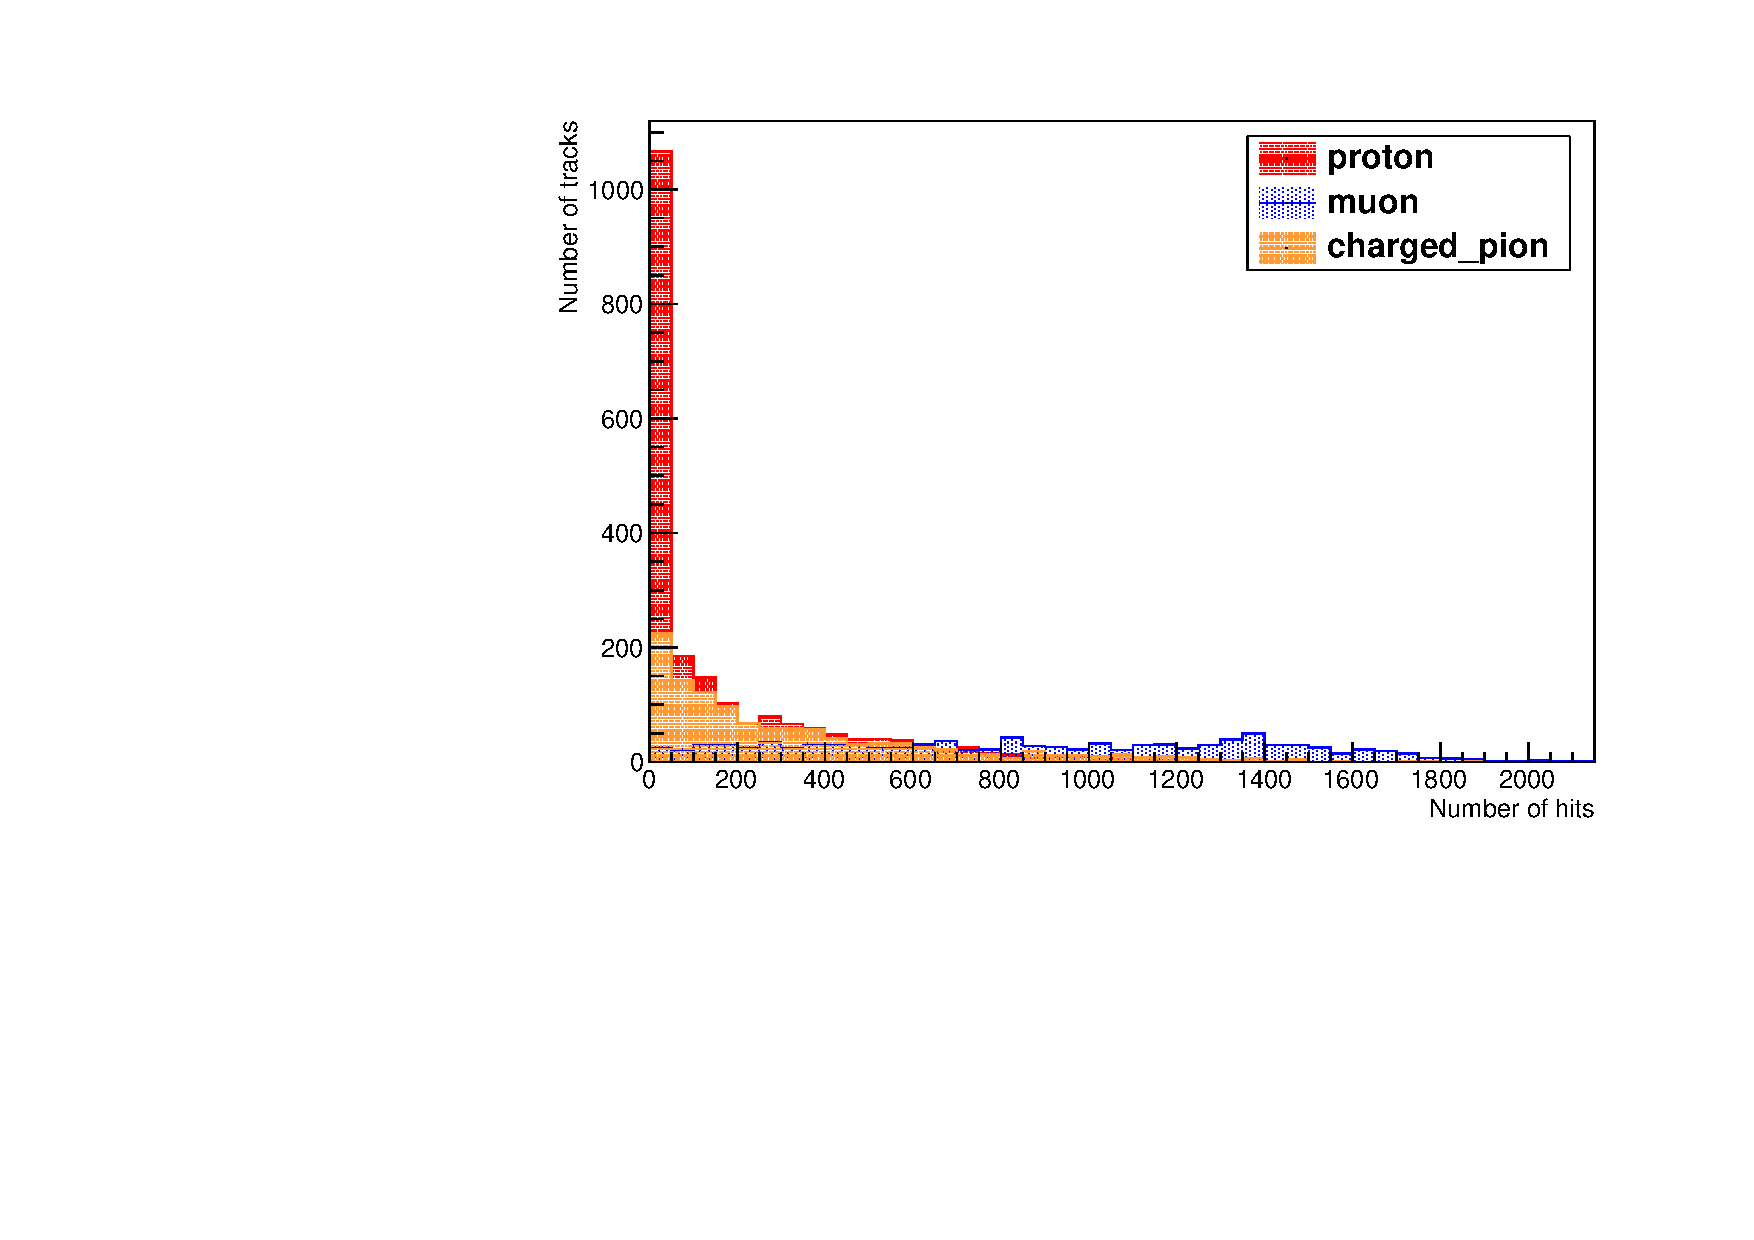
\includegraphics[angle=-90,width=\textwidth]{chapters/particleid_images/ccpi-770-track-lengths}
\caption[Track length distribution for $\mu$ and $p$ from $770\MeV$ neutrinos(CCPi)]{\label{fig:ccpi-track-lengths-770MeV}Distribution of track lengths, represented as number of hits contained in a track, for muon (blue) and proton (red) tracks produced in charged current interactions of $\nu_\mu$ at $770\MeV$ resulting in $\mu + p + \pi^+$ final states. More than $1000$ proton tracks are present, indicating that the $\pi^+$ sometimes produces one or more protons. The distributions are not clearly separated, and while muon tracks are still typically long, there is much more contamination from the other particle species.}
\end{figure}

\begin{figure}
\centering
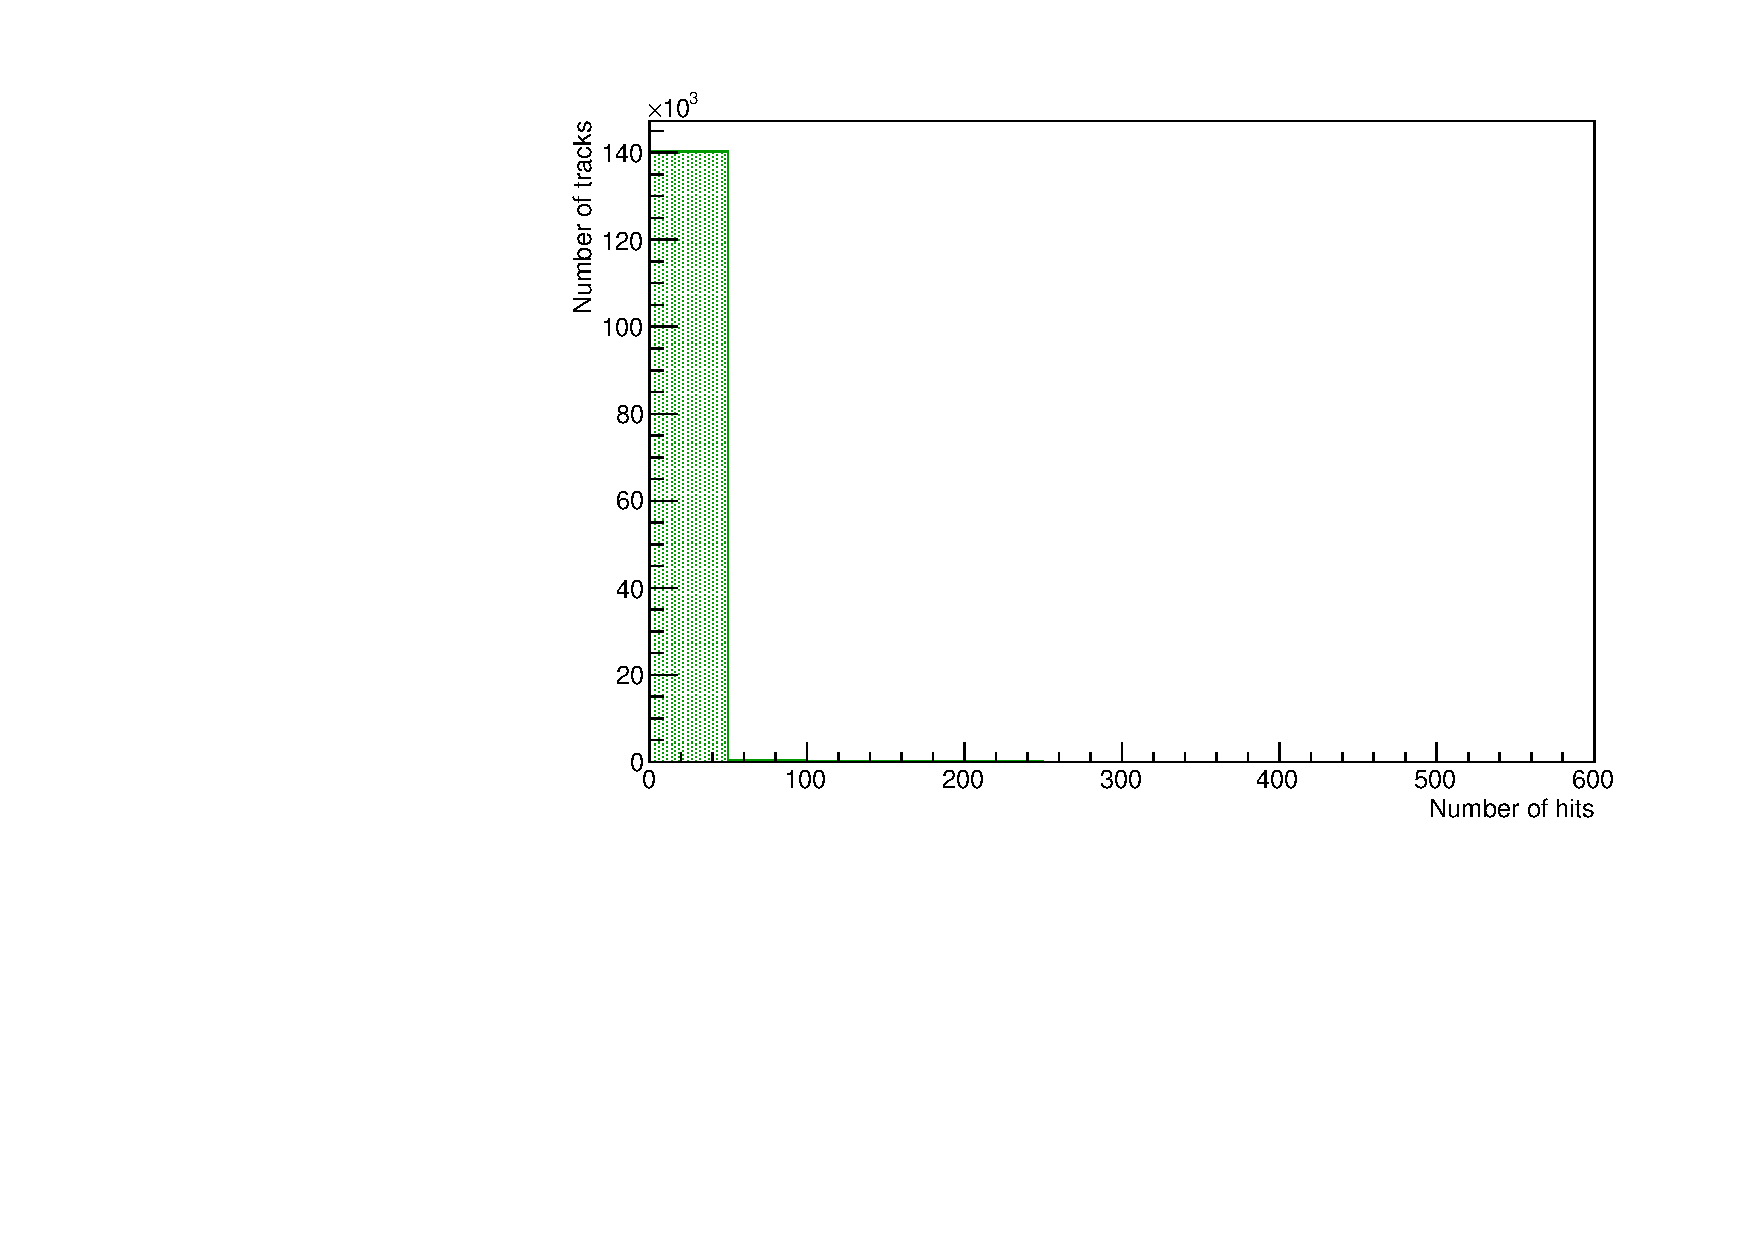
\includegraphics[angle=-90,width=\textwidth]{chapters/particleid_images/ccpi-770-electron-lengths}
\caption[Track length distribution for $e^{-}$ from $770\MeV$ neutrinos (CCPi)]{\label{fig:ccpi-electron-lengths-770MeV}Distribution of track lengths, represented as number of hits contained in a track, for electron tracks produced as secondary particles following charged current interactions of $\nu_\mu$ at $770\MeV$ resulting in $\mu + p + \pi^+$ final states. An extremely large number of very short electron tracks can be seen, corresponding to the production of delta electrons along the length of the trajectories of the primary muon and proton. Most electron tracks have fewer than 50 hits.}
\end{figure}

\subsection{$4.5\GeV$ $\nu_\mu \rightarrow \mu + p$ (CCQE) Interactions}
This data set contains $10^4$ events in which a $4.5\GeV$ $\nu_\mu$ underwent a charged current interaction with an Argon nucleus, producing a $\mu + p$ final state. The distribution of track lengths (represented in terms of the number of hits) for muons, protons and charged pions (which are produced as secondary particles, in these events) is shown in figure \ref{fig:ccqe-track-lengths-4500MeV}. In addition, a large number of short electron tracks are present, the longest containing only $1238$ hits (in contrast, the muon peak is at 22000 hits).

\begin{figure}
\centering
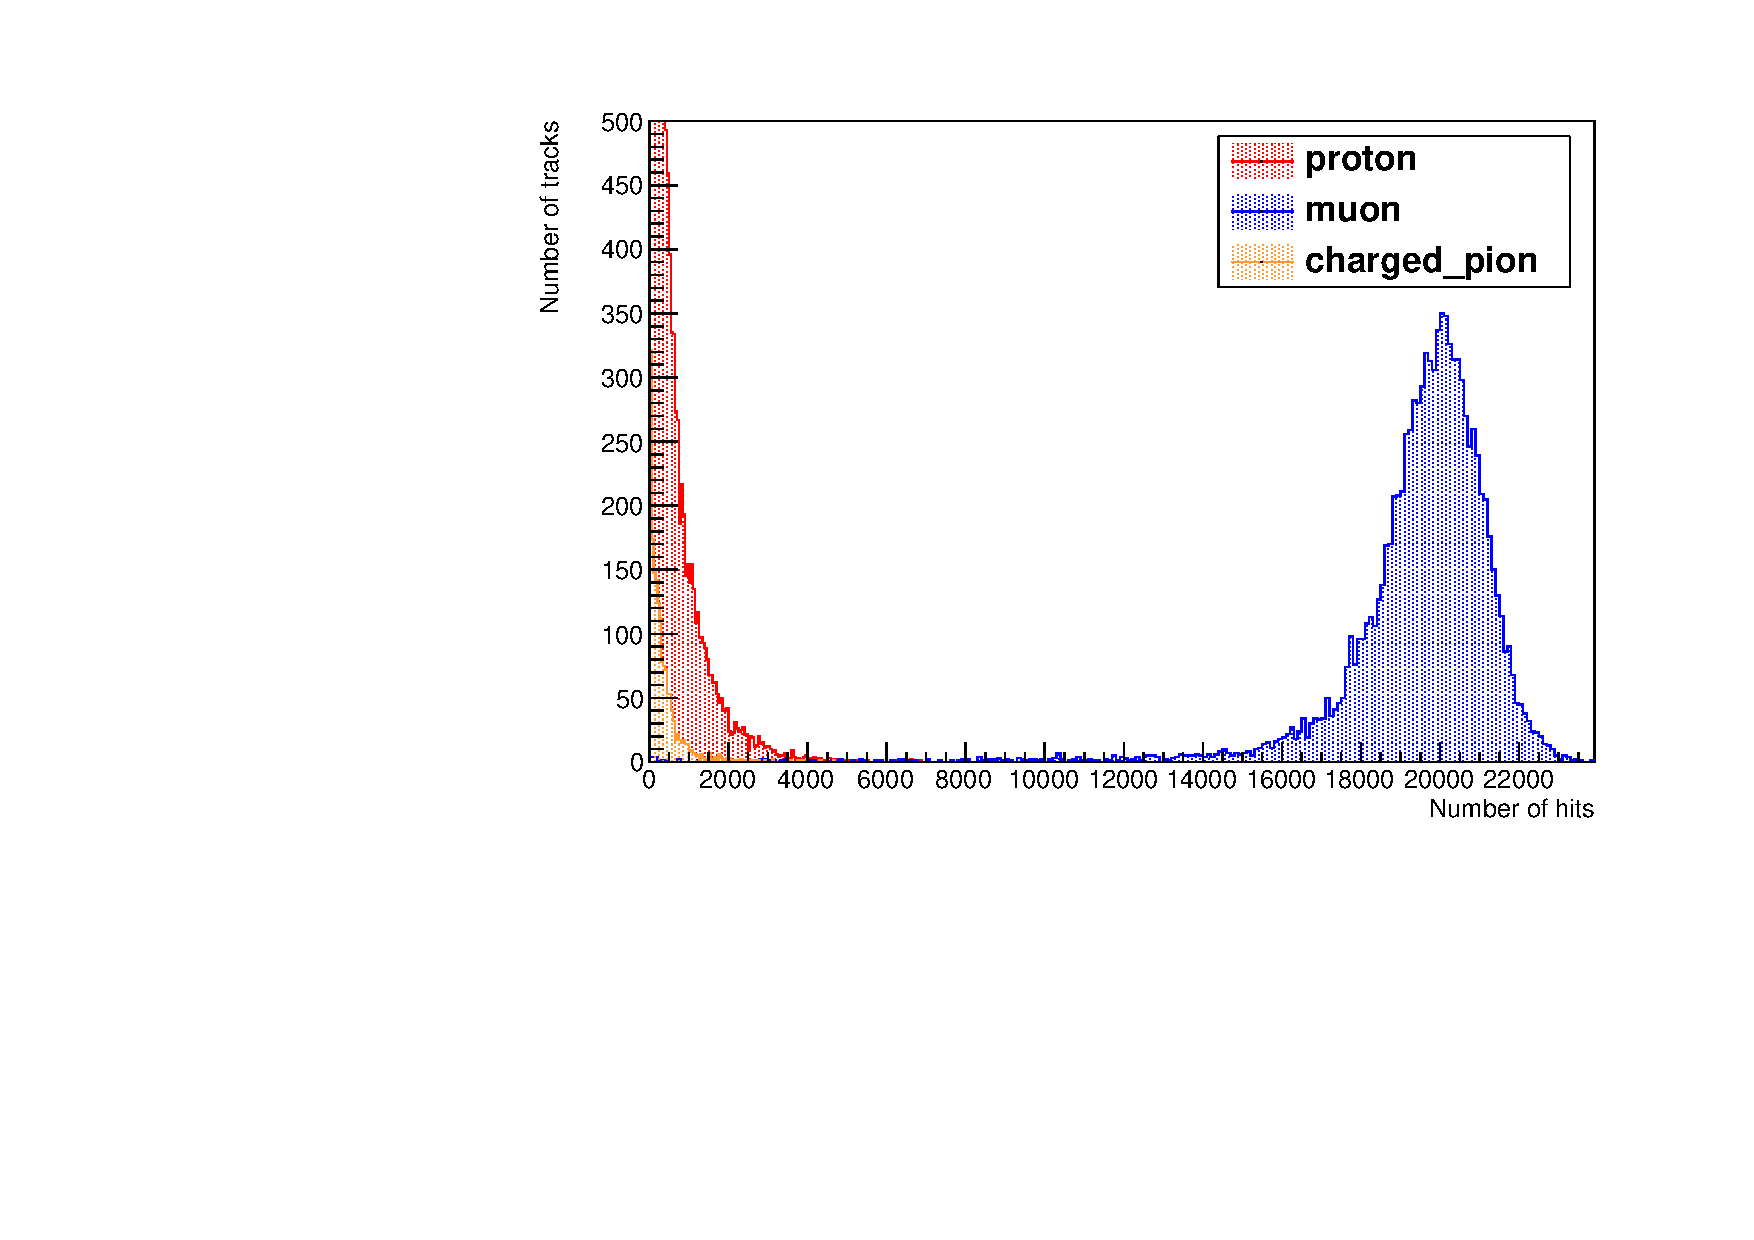
\includegraphics[angle=-90,width=\textwidth]{chapters/particleid_images/ccqe-4500-track-lengths}
\caption[Track length distributions for $\mu$, $p$ and $\pi^+$ from $4.5\GeV$ neutrinos (CCQE)]{\label{fig:ccqe-track-lengths-4500MeV}Distribution of track lengths, represented as number of hits contained in a track, for muon (blue), proton (red) and charged pion (orange) tracks produced in charged current interactions of $\nu_\mu$ at $4.5\GeV$. The proton distribution peaks at over $1.55\times10^4$ tracks on the left.}
\end{figure}

For these high energy events, it is clear that any track with more than around 5000 hits must correspond to a muon, and the vast majority of muon tracks have between 14000 and 24000 hits. Using the track length to separate muons from other particles should provide an extremely pure selection of muons, in this case.

\subsection{$4.5\GeV$ $\nu_\mu \rightarrow \mu + p + \pi^+$ (CCPi) Interactions}

